% This is samplepaper.tex, a sample chapter demonstrating the
% LLNCS macro package for Springer Computer Science proceedings;
% Version 2.21 of 2022/01/12
%
\documentclass[runningheads]{llncs}
%
\usepackage[T1]{fontenc}
% T1 fonts will be used to generate the final print and online PDFs,
% so please use T1 fonts in your manuscript whenever possible.
% Other font encondings may result in incorrect characters.
%
\usepackage{graphicx}
% Used for displaying a sample figure. If possible, figure files should
% be included in EPS format.
%
% If you use the hyperref package, please uncomment the following two lines
% to display URLs in blue roman font according to Springer's eBook style:
%\renewcommand\UrlFont{\color{blue}\rmfamily}
%
\usepackage{orcidlink}

%\usepackage[backend=biber,style=numeric,sortcites,sorting=nty,backref,natbib,hyperref]{biblatex}

%\addbibresource{ref.bib}
\usepackage{float}
\usepackage{booktabs}
\usepackage{arydshln}
\usepackage{amsmath}

\usepackage{pgfplots}
\pgfplotsset{compat=1.17}
\begin{document}
%
\title{Optimized Frequency Regularization: Decrease the Usage of Random Access Memory on Android Devices\thanks{Supported by University of Alberta.}}
%
%\titlerunning{Abbreviated paper title}
% If the paper title is too long for the running head, you can set
% an abbreviated paper title here
%
\author{Wenhao You\inst{1}\orcidlink{0009-0008-3267-5674} \and
Leo Chang\inst{2}\orcidlink{0009-0006-1497-7279} \and
Guanfang Dong\inst{3}\orcidlink{0000-0001-9300-2125} \and
Anup Basu\inst{4}\orcidlink{0000-0002-7695-4148}}
%
\authorrunning{W. You et al.}
% First names are abbreviated in the running head.
% If there are more than two authors, 'et al.' is used.
%
\institute{
University of Alberta, Edmonton, Canada\\
\email{\{wyou1,chewei\}@ualberta.ca}}
%
\maketitle              % typeset the header of the contribution
%
\begin{abstract}
We implemented a compressed algorithm frequency regularization (FR) on Android devices successfully and also packaged frequency regularization into a Python library, being deployed on Android devices. Moreover, we proposed \textbf{few optimized methods of frequency regularization algorithm} to \textbf{reduce the usage of random access memory (RAM)}. Furthermore, we developed a software on Android, implementing frequency regularization and its optimized versions. And we utilized Termux for deploying the frequency regularization Python library on mobile devices. Additionally, we adopted a layer-by-layer memory-freeing approach to optimize the neural network process in the optimized version. We also divided a complete image into four different parts for separated neural network processing. Our experiments in this paper illustrated that \textbf{the layer-by-layer memory-freeing method} works, reducing the usage of random access memory on Android devices significantly. It makes an increasingly possible to deploy certain useful and complex neural networks for image segmentation on limited hardware devices such as mobile phones.

\keywords{Frequency regularization  \and Neural network optimization \and Python library \and Random access memory \and Android devices.}
\end{abstract}
%
%
%
\section{Introduction}

Currently, people cannot live without mobile devices. They are not only for communication and entertainment, the information transformation is also a significant feature. Their portability and versatility make them play an important role in our daily lives. Meanwhile, convolutional neural networks (CNNs) are also vital in some research areas such as computer vision and other interdisciplinary data analysis. However, these neural networks are usually implemented on high-end hardware because of their huge amount of parameters and layers. It means that only a few researchers work on the deployment of neural networks on mobile. There exists several advantages of running convolutional neural networks on mobile devices: privacy, internet, and runtime. First, personal information does not need to be uploaded or transmitted to the cloud servers which improves the privacy enhancement. Second, the functionality on local devices can replace some internet services. Therefore, it is independent from the internet connection. Last, in some applications that need real-time feedback, without connecting to the cloud server can shorten the processing time which decrease the runtime. In all, convolutional neural networks can totally replace the usage of many applications on mobile devices, ensuring personal data security. %??

According to the popularity of mobile devices and the benefits of convolutional neural networks, we want to find a way to deploy some large and complex convolutional neural networks on mobile devices, leading to the question: ``How can we deploy large convolutional neural networks on mobile devices?''

We found five methods to achieve our goal: upgrade the hardware to a high-specification mobile device; implement Extreme Learning Machine (ELM)~\cite{anton2021elm} to allocate the weight of hidden layers randomly in order to train large models on mobile devices faster; implement NestDNN~\cite{fang2018nestdnn} dynamically adjusts the size and computational complexity of the network based on available resources on mobile devices; implement ``One-shot Whole Network Compression''~\cite{kim2016oneshot} to prune, quantize, and compress the neural networks; implement frequency regularization (FR)~\cite{zhao2023fr} algorithm to reduce parameters by removing high-frequency component. We make a more detailed introduction to their drawbacks and limitations in Section~\ref{related_work}.

After conducting a thorough literature review, considering all the limitations, accuracy, complexity, and future potential, we choose frequency regularization (FR) as our target algorithm. We deployed it on the Android-based device which is one of the most popular operating system on mobiles. Our main idea is to implement FR to compress a U-Net convolutional neural network and then decompresses the uploaded compressed model on an Android mobile device in a short time. After that, take the decompressed model to do image segmentation for the Carvana Image Masking Challenge Dataset~\cite{brian2017carvanadataset}. 

\begin{figure}[htbp]
	\centering
	\label{image:workflow}
	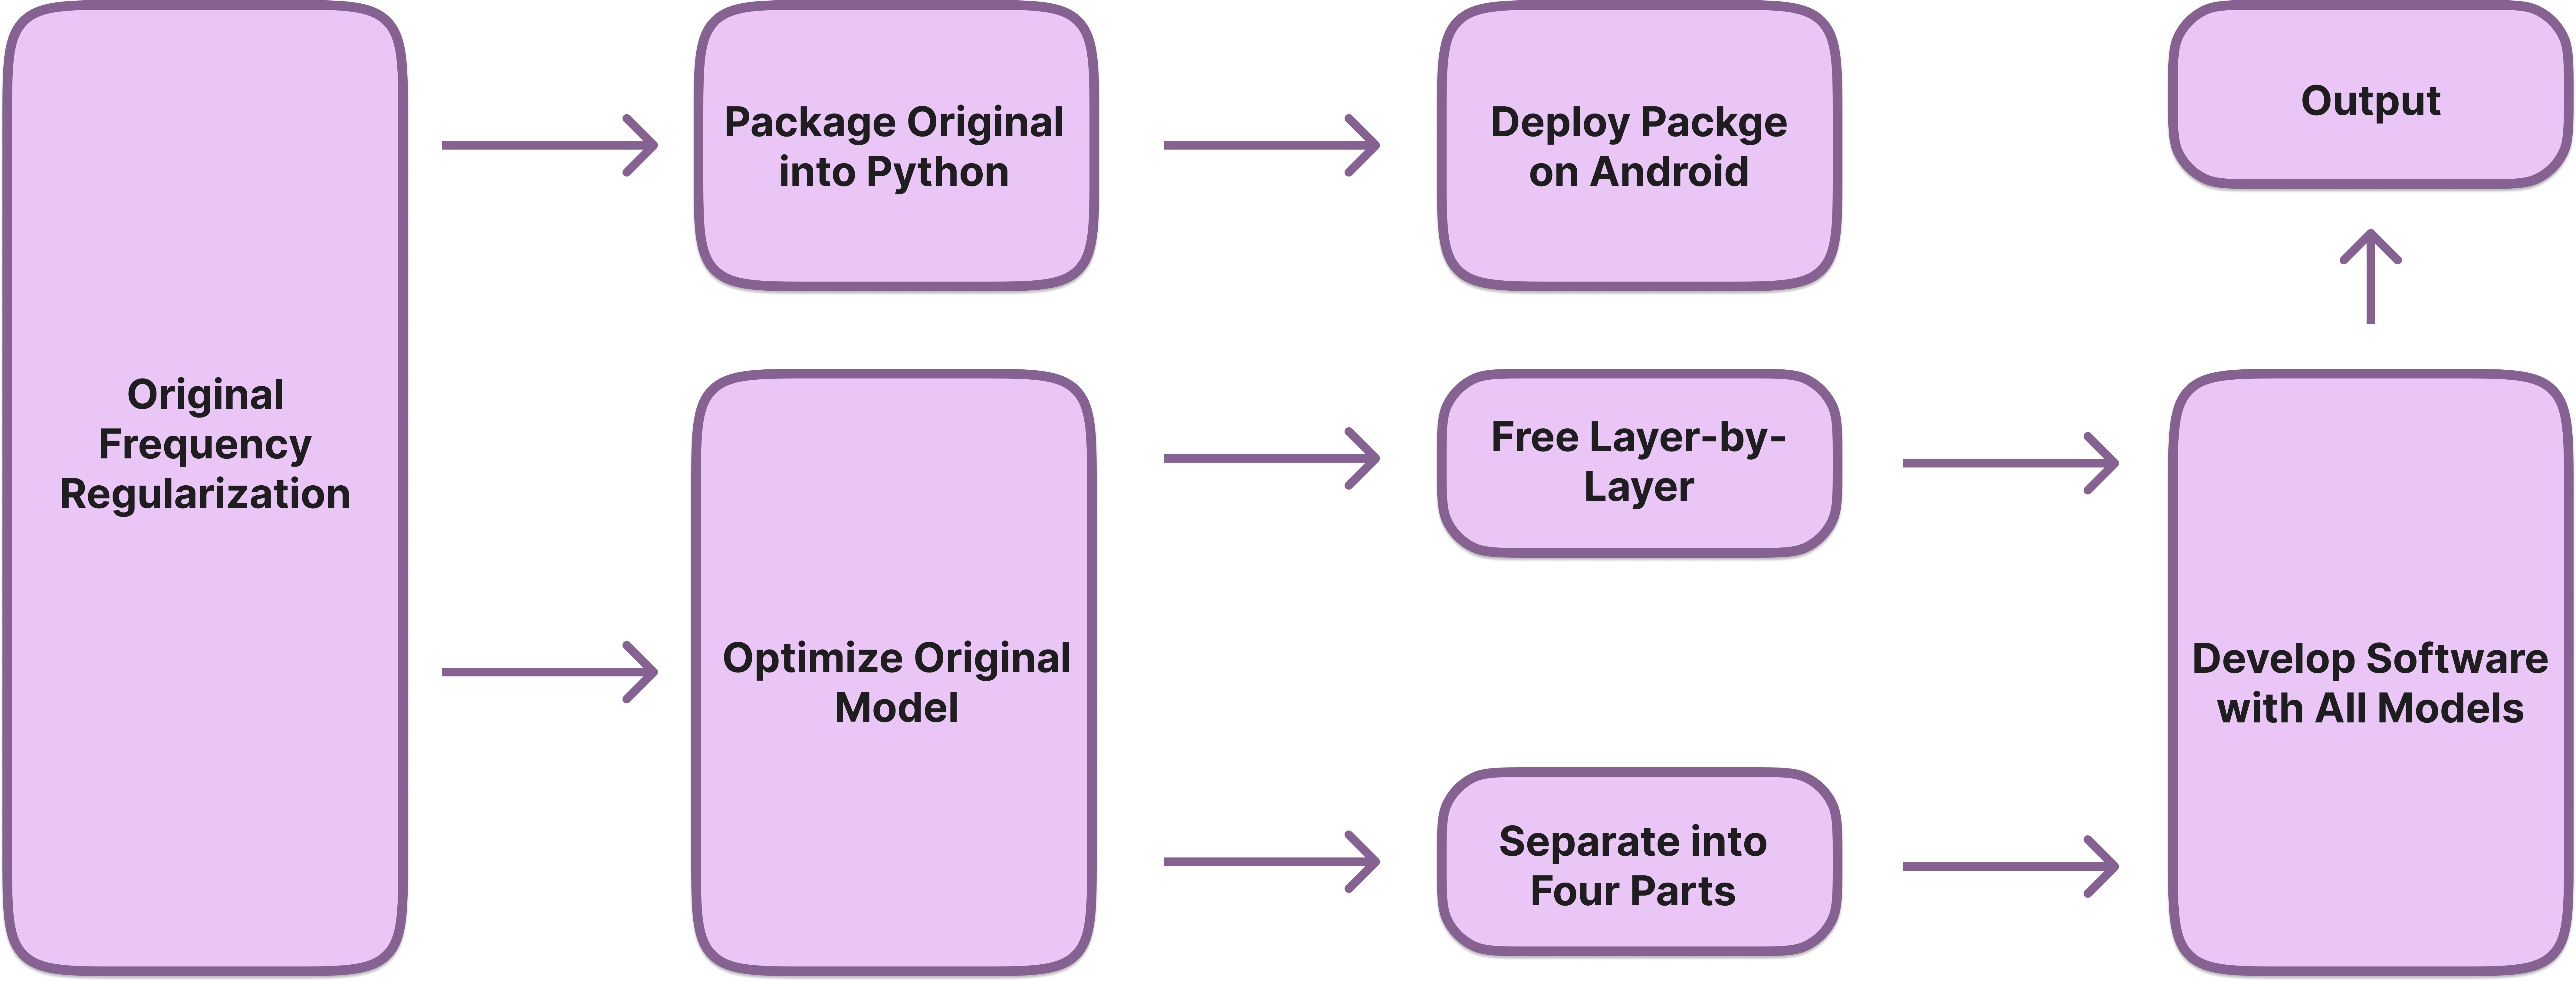
\includegraphics[width=1\linewidth]{figures/workflow.jpg}
	\caption{General workflow of deploying frequency regularization and its optimized versions on Android devices.}
\end{figure}

In our work, before optimizing the existing FR code~\cite{fr_repo}, we have two different directions of implementing the program on a mobile device. One is to install the Linux virtual environment by using Termux~\cite{termux_repo},~\cite{termux_overview},~\cite{termux_wiki} on the Android system and to deploy the source code implementation. Another one is to develop an Android application which contains the code of frequency regularization by using Android Studio. As shown in Fig.~\ref{image:workflow}, our workflow also contains the optimization/improvement of existing frequency regularization~\cite{zhao2023fr},~\cite{fr_repo}. The approach of freeing RAM layer-by-layer decreases the total usage of RAM on Android phones significantly. Moreover, the output quality of image segmentation does not have any side effects. Overall, our main contributions are:
\begin{enumerate}
	\item Packing the frequency regularization source code into the Python library and installing it on the Android system successfully.
	\item Optimizing and improving the existing frequency regularization algorithm to decrease the RAM usage on mobile devices.
	\item Developing Android application containing original frequency regularization algorithm and all the other optimized versions to apply image segmentation.
\end{enumerate}

Our optimized models achieve the RAM usage around $1.932$ GB whereas the RAM usage of original frequency regularization algorithm is around $3.270$ GB on Android devices. This means the optimized models are $40.9\%$ relative improvements over previous algorithm~\cite{zhao2023fr},~\cite{fr_repo} specially for Android devices. %??



\section{Related Work}\label{related_work}
There are four main related works in this Section: Extreme Learning Machine (ELM)~\cite{anton2021elm},~\cite{ding2014elmapp},~\cite{wang2022elmapp},~\cite{deng2015elmapp},~\cite{huang2006elmapp}, NestDNN~\cite{fang2018nestdnn}, ``One-shot Whole Network Compression''~\cite{kim2016oneshot}, and Frequency Regularization~\cite{zhao2023fr},~\cite{fr_repo}. 

Extreme learning machine (ELM) has been widely used in artificial intelligence field over the last decades~\cite{anton2021elm},~\cite{ding2014elmapp},~\cite{wang2022elmapp},~\cite{deng2015elmapp},~\cite{huang2006elmapp}. Although this algorithm has seen significant development, it also contains several drawbacks. It is also the reason that we do not use ELM in our work: 
\begin{itemize}
	\item Poor tunability: It has poor controllability of the model since ELM calculates the least squares solution directly, and users cannot analyze the characteristics of the datasets to fine-tune. Adjusting models based on the specific performance of mobile devices is important to mobile development.
	\item Lack of robustness: The performance of the model can be affected significantly while including certain outliers in different datasets, indicating poor robustness. Deployment on mobile devices needs to handle various inputs, including every potential outlier. Although there are many advanced versions of ELM~\cite{john2015advancedelm},~\cite{zhang2015advancedelm},~\cite{zhu2005advancedelm},~\cite{sun2017advancedelm} they lack universality and are not as easy as other algorithms to deploy.
	\item Overfitting issues: While deploying large convolutional neural networks on mobile devices, model generalization is crucial since overfitting can result in poor performance on unseen data. ELM easily leads to overfitting issues because it is based on empirical risk minimization without considering structural risk. Xue et al.~\cite{ying2019overfit}pointed to a regularization strategy to solve this problem by feature selection.
\end{itemize}	 

NestDNN is a framework that takes the dynamics of runtime resources into account~\cite{fang2018nestdnn}. The experiment of Fang et al.~\cite{fang2018nestdnn} achieves as much as $4.2\%$ increase in inference accuracy, $2.0\times$ increase in video frame processing rate and $1.7\times$ reduction in energy consumption. However, NestDNN also comes with some limitations. Its computational cost is significantly higher by using filter pruning method Triplet Response Residual (TRR). The high computational cost could probably exceed the processing capabilities of existing mobile devices and the runtime of model generation may be too long, which is not suitable for our deployment. 

``One-shot Whole Network Compression''~\cite{kim2016oneshot} includes removing certain parameters or structures, which is irreversible. Moreover, by using this compression method, the accuracy is too low. For example, in the experiment of Kim et al., by using AlexNet, the accuracy of the compressed model can drop by more than $50\%$. In order to increase its accuracy, we have to fine-tune the compressed model. Increasing accuracy requires at least more than $10$ training epochs, which takes too much time. In our work, to deploy on mobile devices, this algorithm cannot be chosen obviously. 


Frequency regularization (FR)~\cite{zhao2023fr},~\cite{fr_repo} works by restricting the non-zero elements of network parameters in the frequency domain, thus reducing information redundancy. Table~\ref{table:fr_unet} illustrates the evaluation of the proposed frequency regularization algorithm on UNet, according to compression rate, number of parameters, and dice score. Dice score is a metric for assessing the quality of image segmentation and ranges from $0$ to $1$, where $0$ indicates no overlap and $1$ indicates perfect overlap. The data under the dashed-line represents the result under the most extreme condition in which only $759$ float$16$ parameters are kept in UNet-v$4$. Thus, according to the surprising and satisfying experiment outcomes, we chose frequency regularization as our compression method to do further implementation, to deploy it on mobile devices (i.e. Android system).

\begin{table}[H]
	\caption{Evaluation of the proposed frequency regularization algorithm on UNet for image segmentation tasks using Carvana Image Masking Challenge Dataset~\cite{zhao2023fr},~\cite{brian2017carvanadataset}.} 
	\label{table:fr_unet}
	\small
	\centering
	\begin{tabular}{rrrr}
		\toprule
		&Dice Score&Compression Rate&\# of Parameters\\ 
		\midrule\midrule
		UNet-ref&99.13\%&100\%(1×)&31,043,586\\
		UNet-v1&99.51\%&1\%(100×)&310,964\\
		UNet-v2&99.37\%&0.1\%(1000×)&31,096\\
		UNet-v3&98.86\%&0.0094\%(10573×)&2,936\\
		\cdashline{1-4}
		UNet-v4&97.19\%&0.0012\%(81801×)&759(float16)\\
		\bottomrule
	\end{tabular}
\end{table}

\section{Methodology}\label{methodology}
\subsection{Problem Formulation}~\label{formulation}
To implement frequency regularization algorithm~\cite{zhao2023fr},~\cite{fr_repo} on Android devices effectively, our primary goal is to optimize the algorithm in order to reduce the usage of random access memory (RAM). In our work, we chose image segmentation to test the efficiency of the methods. The optimization we want to achieve is ensuring that the devices run the algorithm efficiently without compromising lots of available memory resources. Simultaneously, there is another problem we need to solve: maintain the quality of results as much as possible while optimizing the algorithm. The balance between memory efficiency and the quality of images is the key to deliver an optimized user experience on mobile devices. The challenges in our work involve adjusting the algorithm to minimize the RAM usage while preserving the integrity and clarity of the processed images (i.e. image segmentation in our work).


\subsection{Original and Optimized Frequency Regularization}~\label{optimized}
To carry out the experiment of image segmentation, we designed two creative methods based on frequency regularization algorithm~\cite{zhao2023fr},~\cite{fr_repo}  to optimize the usage of memory and its efficiency. We also want to make sure that the accuracy is still effective after the optimization.
\begin{itemize}
	\item Original frequency regularization: In Section~\ref{related_work}, Zhao et al. designed this method and we will use their source code~\cite{fr_repo} to implement it on the Android system.
	\item Free random access memory layer-by-layer based of the neural network: In this method, we stored the tensor information of the network layers in the local storage and free the random access memory (RAM) while each layer ends. 
	\item Free random access memory layer-by-layer of the neural network and separate one image into four parts: The main idea is similar to the previous method. We planned to separate an image into four different parts and implement the previous method on each four parts independently. After that, we merge the four parts together to get the result. 
\end{itemize}	 		

\subsection{Deployment Tools}~\label{deployment}
To deploy all the frequency regularization related methods in Section~\ref{optimized} on Android devices, we have two different implementations. In other words, we have to use two different tools. One is Termux, which can implement a Linux virtual environment on an Android system. The other is Android Studio, which can help to develop Application with FR image segmentation.
\begin{itemize}
	\item Termux~\cite{termux_repo},~\cite{termux_overview},~\cite{termux_wiki}  is a terminal application so that we can run the Linux virtual environment. It only requires some minimum setups. However, to run Termux, the system needs to meet some minimal requirements: Android $5.0$ to $12.0$; CPU: AArch$64$, ARM, i$686$, x$86\_64$; at least $300$ MB of disk space. It is open source and its documentation can be accessed at the link \href{https://github.com/termux/termux-app}{here}. The instruction of installing Termux on Android devices is available at \href{https://github.com/btxcy/NeuralOnMobile\#readme}{here}. 
	\item Android Studio is an Integrated Development Environment (IDE) designed specifically for developing applications for the Android platform. Moreover, this platform supports the PyTorch Mobile Library, which makes it to be more simple to deal with neural networks on Android system.
\end{itemize}	 		

\subsection{Qualitative and Quantitative Metrics}~\label{metrics}
To analyze the results of our experiment, we have three qualitative and quantitative metrics: usage of random access memory, dice score, and visual perception. In our work, we need to analyze these three metrics collectively rather than making judgments on them individually.
\begin{itemize}
	\item Usage of Random Access Memory (RAM): The RAM usage is a key metric when evaluating the performance of any software application. RAM usage usually refers to the amount of memory that the system allocates to a particular task or application while it is running. This quantitative metric reflects the demand for computing resources, as well as its efficiency. The lower usage of RAM is used, the higher efficiency of the application. In Section~\ref{experiments}, we tried to decrease the RAM usage in order to avoid unnecessary waste of resources and allow more lower-end Android devices to deploy the neural networks.
	\item Dice Score: It is also known as the Dice Similarity Coefficient. It is a measure of the similarity between two sets of data, usually represented as binary arrays~\cite{dicescore2023}. For example, in the image segmentation of Section~\ref{experiments}, the dice score can be used to evaluate the similarity between a predicted segmentation mask and the ground truth segmentation mask~\cite{dicescore2023}. Its range is betweem $0$ and $1$, representing no overlap to perfect overlap. The higher value the more closer to the ground truth. We used this quantitative method to evaluate the performance of the algorithms. Equation \eqref{eq:dice} shows the formula of dice score~\cite{yerram2020dice}.
	
	\begin{equation}\label{eq:dice}
		\text{Dice Score} = \frac{2 \times |X \cap Y|}{|X| + |Y|}
	\end{equation}
\\where X is the predicted set of pixels and Y is the ground truth.\\
		\item Visual Perception: Visual perception as a metric in image quality assessment involves evaluating images based on how well they align with human visual characteristics~\cite{fu2016visual}. Though numerous image quality measures have been proposed, human visual perception is still a good way to evaluate the quality of images~\cite{wajid2014visual}. In all, we used our own perception as a qualitative metric and combined it with the other two quantitative metrics to decide the best outcomes in our experiment. 
\end{itemize}	



\section{Experiments} ~\label{experiments}
\subsection{Experimental Settings}
We utilized an Android device that ran version $12.0.1$ and $8$ GB RAM for this section. In order to facilitate the installment of Ubuntu operating system within the Android system, we downloaded Termux~\cite{termux_repo},~\cite{termux_overview},~\cite{termux_wiki}, which version is v$0.118.0$. Upon accessing Termux, we employed a suite of basic tools, such as wget, proot, and git, to establish the Ubuntu. The Ubuntu package~\cite{ubuntu_in_termux_repo} we used is quite different from the conventional Ubuntu installations on normal personal computers. For more detailed steps of setting up the environment, please check our source code repository~\cite{nerual_on_mobile_repo}. For developing the Android Application, we utilized the same version of the emulator (i.e. Android Virtual Device) and made sure that the Android Studio we chose is in version $2023.1.1$. The detailed steps can be checked on our source code repository as well~\cite{nerual_on_mobile_repo}.


\subsection{Package Frequency Regularization Source Code}~\label{package_fr}
As of the current and future plans of Zhao et al.~\cite{fr_repo},~\cite{zhao2023fr}, we have accomplished \textbf{the development of a pip repository for their frequency regularization technique} and committed to their original repository~\cite{fr_repo}. We can now integrate frequency regularization algorithm into our project by simply running the command line in the Linux virtual environment: \texttt{\$ pip install frereg}. This step is instrumental in simplifying the deployment of condensed yet potent models in pragmatic applications. We will use this Python library in Section~\ref{build_linux}.

\subsection{Build Linux Virtual Environment and Install the Frequency Regularization Library} ~\label{build_linux}
After initiating the Ubuntu operating system~\cite{ubuntu_in_termux_repo} and installing both Python and the Python-pip tool, we used the command line mentioned in Section~\ref{package_fr} and installed the frequency regularization library successfully. From our own perspectives, this method is not that innovative since it is based on the Termux, which is a mature Linux virtual environment for Android system. This part of our experiment aims to \textbf{prove the possibility of running a compressed model by building a Linux environment}, that only requires enough random access memory (RAM).


\subsection{Develop an Application with Optimized Methods}~\label{deploy_as}
As mentioned in Section~\ref{methodology}, we utilize Android Studio to develop an application with our methods. In order to run the Python script on the Android Studio, there is a library called Chaquopy~\cite{chaquopy2023} that can help us. Our Android application can upload the chosen images from local storage and implement the original frequency regularization or the other optimized methods respectively. We use this application to generate all the data we need in this research, such as the usage of RAM. We also use this application to obtain the outputs from the algorithm and its optimized version running on an Android phone. The feature of the application provides currently include importing an image from the local machine directory and running a bulk of images in one run. After that, we get the output from the compressed algorithm and store it in the local device automatically.

\subsection{Analyze Results}
Fig.~\ref{image:3_outputs} illustrates the results among three ways of image segmentation. The left-hand column of the Fig.~\ref{image:3_outputs} shows the original images we want to implement the image segmentation. From left to right, the three columns represent three outputs generated by an Android phone respectively: output from non-optimized code, output from optimized code, output from optimized code and separate the original image into 4 parts. 
\begin{figure}[htbp]
	\centering
	\label{image:3_outputs}
	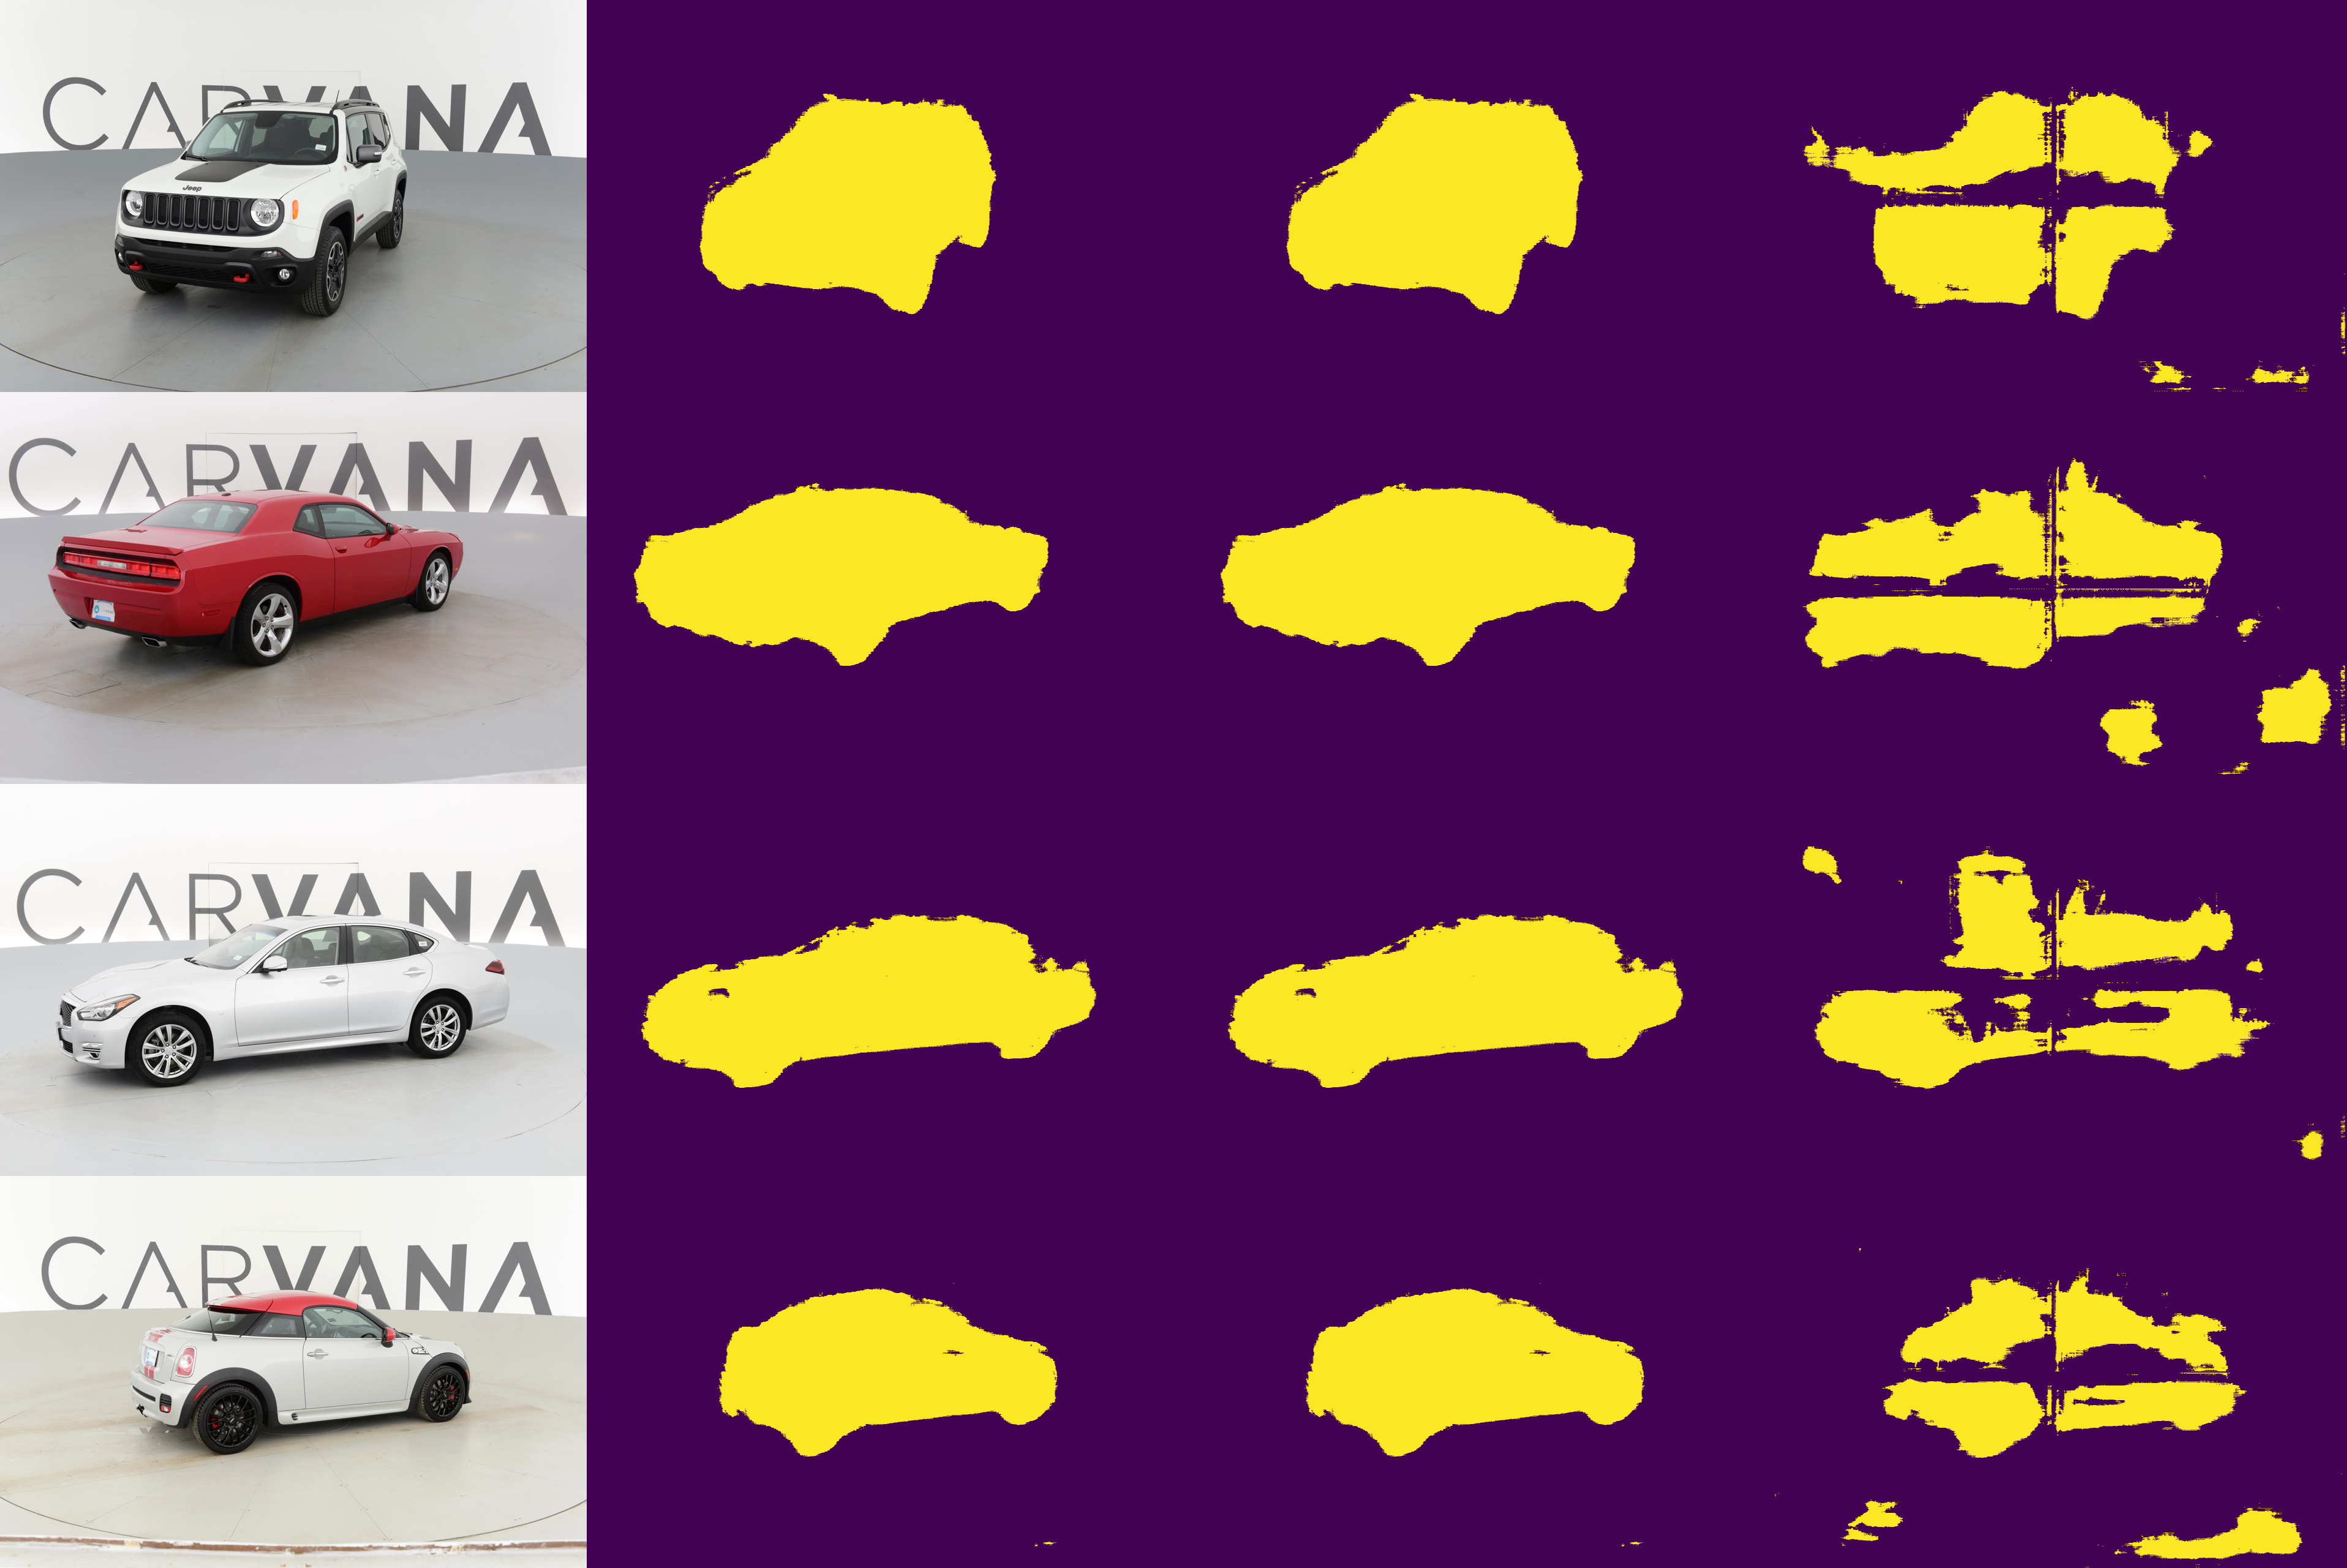
\includegraphics[width=0.8\linewidth]{figures/3_outputs.png}
	\caption{Comparison between Original Images and Outputs from Image Segmentation for Carvana Image Masking Challenge Dataset~\cite{brian2017carvanadataset} on an Android Phone: Uncompressed U-Net, FR Compressed and Decompressed U-Net, and FR Compressed and Decompressed U-Net Processing Four Parts of an Image Simultaneously.}
\end{figure}

 Table~\ref{table:ram_usage} shows that the average RAM usages among three experiments are $3.2687$ GB, $1.9318$ GB, and $1.3063$ GB respectively. It is obvious that the optimized frequency regularization algorithm \textbf{decreases the RAM usage on Android devices significantly}. Because of this, we will say that more Android phones equips lower-end hardware can probably implement these two algorithms. To analyze Table~\ref{table:dice_score}, the table illustrates the average dice scores among three experiments. For using the compressed model (i.e. FR) directly, the dice score is $0.9718$ which is identical as using the original non-compressed model. Moreover, for using the compressed model on four separated parts of the image, the dice score shows a small number of $0.7567$, which means that the image segmentation under this method does not output a good quality. Combining these two tables: Table~\ref{table:ram_usage} and Table~\ref{table:dice_score}, and the visual perception in Fig.~\ref{image:3_outputs}, using FR directly on Android is a better algorithm to implement on the U-Net. Obviously, the original compressed model and optimized compressed model by FR have almost the same quality of image segmentation. By visual perception, we are more certain that \textbf{optimized FR is a highly efficient algorithm} even if the system is Android.


\begin{table}[H]
	\caption{Comparison of Usages of RAM for Image Segmentation for Carvana Image Masking Challenge Dataset~\cite{brian2017carvanadataset} on an Android Phone: Original FR, Free RAM Layer-by-Layer of neural network, and Free RAM Layer-by-Layer of neural network with Four Separate Parts in Section~\ref{methodology}.} 
	\label{table:ram_usage}
	\small
	\centering
	\setlength{\tabcolsep}{10pt}
	\begin{tabular}{rrrr}
		\toprule
		& Original & Optimized & Optimized \& 4 parts\\
		\midrule\midrule
		1$^{st}$ Avg.&3.4088 GB&2.0217 GB&1.2684 GB\\
		2$^{nd}$ Avg.&3.1013 GB&1.8294 GB&1.2602 GB\\
		3$^{rd}$ Avg.&3.2959 GB&1.9444 GB&1.3823 GB\\
		\cdashline{1-4}
		Total Avg.&3.2687 GB&1.9318 GB&1.3036 GB\\
		\bottomrule
	\end{tabular}
\end{table}

\begin{table}[H]
	\caption{Comparison of Dice Scores for Image Segmentation for Carvana Image Masking Challenge Dataset~\cite{brian2017carvanadataset} on an Android Phone: Original FR, Free RAM Layer-by-Layer of neural network, and Free RAM Layer-by-Layer of neural network with Four Separate Parts in Section~\ref{methodology}.} 
	\label{table:dice_score}
	\small
	\centering
	\setlength{\tabcolsep}{10pt}
	\begin{tabular}{rrrr}
		\toprule
		& Original & Optimized & Optimized \& 4 parts\\
		\midrule\midrule
		1$^{st}$ Avg.&0.9718&0.9718&0.7567\\
		2$^{nd}$ Avg.&0.9718&0.9718&0.7567\\
		3$^{rd}$ Avg.&0.9718&0.9718&0.7567\\
		\cdashline{1-4}
		Total Avg.&0.9718&0.9718&0.7567\\
		\bottomrule
	\end{tabular}
\end{table}


\section{Limitation}
\subsection{Incomplete Mobile PyTorch}
In some situations, some PyTorch features may still not work when running the code because of the difference in hardware structure between the computer and mobile devices~\cite{fojtik2022cpu}. For instance, the Discrete Fourier Transforms or the Fast Fourier Transforms~\cite{james1996dft},~\cite{cochran1967dft},~\cite{henri1982fft},~\cite{brigham1988fft}, mobile devices do not support this operation due to the requirement of GPU involvement. Therefore, an alternative solution is to convert the tensor data to the NumPy array, which runs through the CPU. After the transformation, we then convert back to the PyTorch tensor array for further steps. Many functions require conversion to make it work in the frequency regularization algorithm. But this approach will decrease the efficiency too much.

\subsection{Unknown Trend}
Fig.~\ref{plot:optimized} shows the trend of RAM usages by using the optimized frequency regularization (i.e. free RAM layer-by-layer). For the three experiments by using the same method, we get the similar trend. It is unexpected since we thought the usage of RAM should keep decreasing while the output of each layers are saved in the local storage. 

\begin{figure}[h]
	\centering
	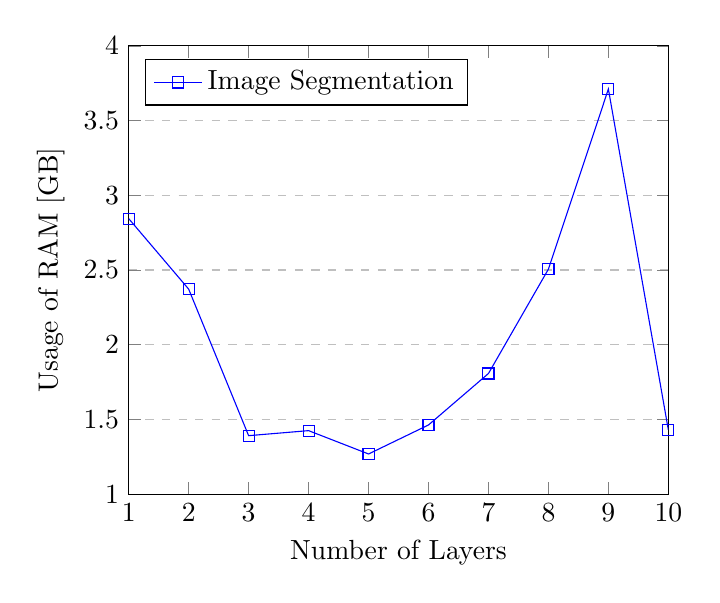
\begin{tikzpicture}
		\begin{axis}[
			xlabel={Number of Layers},
			ylabel={Usage of RAM [GB]},
			xmin=1, xmax=10,
			ymin=1, ymax=4,
			xtick={1,2,3,4,5,6,7,8,9,10},
			ytick={1,1.5,2,2.5,3,3.5,4},
			legend pos=north west,
			ymajorgrids=true,
			grid style=dashed,
			]
			
			\addplot[
			color=blue,
			mark=square,
			]
			coordinates {
				(1, 2.84366848)
				(2, 2.371833856)
				(3, 1.391190016)
				(4, 1.42483456)
				(5, 1.268662272)
				(6, 1.462788096)
				(7, 1.807253504)
				(8, 2.505711616)
				(9, 3.710410752)
				(10, 1.430171648)
			};
			\addlegendentry{Image Segmentation}
			
		\end{axis}
	\end{tikzpicture}
	\caption{Trend of One of the Three Experiments about Optimized Frequency Regularization (i.e. free RAM layer-by-layer) on RAM Usage for Image Segmentation.}
	\label{plot:optimized}
\end{figure}


\section{Future Work}
The main purpose of our future work is to prove the general applicability of frequency regularization algorithm~\cite{zhao2023fr}. We plan to expand more neural network models like ResU-Net, SegNet, X-Net, and so on~\cite{foivos2020resunet},~\cite{vijay2017segnet},\cite{fujii2021xnet}. We also plan to try figuring out the cause of the trend to be not monotonic. Moreover, adjusting and improving frequency regularization to fit more tasks with not only image segmentation is the direction we want to explore. We are also interested in continuing the development of our Android application. Our plan is to enhance this software by adding more models and features, optimizing algorithms, and aiming to make it a more efficient and user-friendly patent.


\section{Conclusion} 
We created \textbf{the first Python library of frequency regularization} and tested it in good condition on the Android system. We also proposed \textbf{few methods of optimizing frequency regularization}\textbf{that helps decreasing the RAM usage without any significant loss}. This creative approach based on Zhao et al. 's frequency regularization algorithm~\cite{zhao2023fr} solved some limitations and improved their work a lot. Moreover, this approach helped us \textbf{deploy it on Android devices} successfully and quickly. To some extent, by using the approach proposed by us, the popularization of using large and complex neural networks on mobile devices will become possible.

\newpage
\bibliographystyle{plain}
\bibliography{ref}


\end{document}
